\documentclass{standalone}
\usepackage{tikz}
\begin{document}
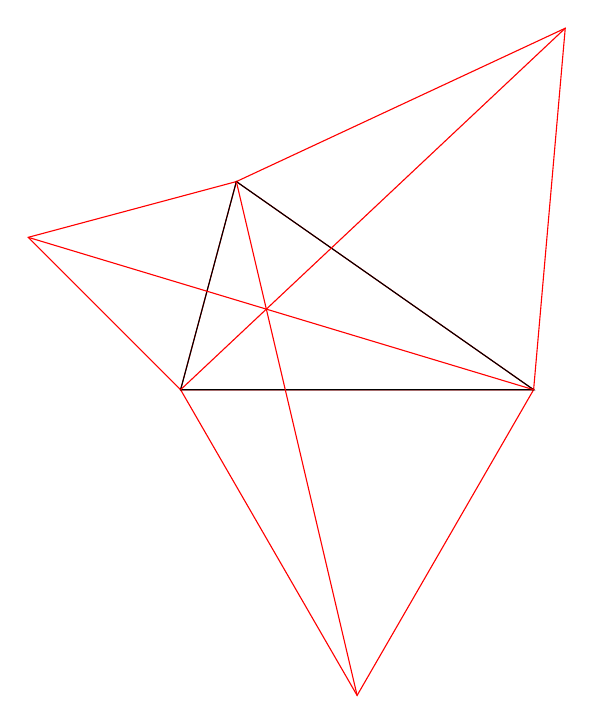
\begin{tikzpicture}[x=1pt,y=1pt]
\draw[red] (90.21,-161.37) -- (153.99,-271.84) -- (217.77,-161.37) -- cycle;
\draw[red] (110.36,-86.16) -- (217.77,-161.37) -- (229.20,-30.75) -- cycle;
\draw[red] (35.15,-106.31) -- (90.21,-161.36) -- (110.36,-86.16) -- cycle;
\draw (110.36,-86.16) -- (90.21,-161.37) -- (217.77,-161.37) -- cycle;
\draw[red] (110.36,-86.16) -- (153.99,-271.84);
\draw[red] (90.21,-161.37) -- (229.20,-30.75);
\draw[red] (217.77,-161.37) -- (35.15,-106.31);
\end{tikzpicture}
\end{document}
